% Created 2023-01-19 Чт 00:16
% Intended LaTeX compiler: pdflatex
\documentclass[PI, VKR]{HSEUniversity}
         \usepackage{array,tabularx,tabulary,booktabs,longtable,multirow}
         \Year{\the\year{}}
         \supervisor{к.т.н., доцент кафедры информационных технологий в бизнесе НИУ ВШЭ-Пермь}{А. В. Бузмаков}
                  \Abstract{В данной работе проведен анализ этичности разных компаний.

В первой главе находится описание используемых алгоримов.

Во второй главе представлено проектирование системы.

В третьей главе представлена реализация системы.

В четвертой главе представлено тестирование работы системы.

Количество страниц - N, количество иллюстраций - N, количетсво таблиц - N.}


\usepackage[utf8]{inputenc}
\usepackage[T1]{fontenc}
\usepackage{graphicx}
\usepackage{longtable}
\usepackage{wrapfig}
\usepackage{rotating}
\usepackage[normalem]{ulem}
\usepackage{amsmath}
\usepackage{amssymb}
\usepackage{capt-of}
\usepackage{hyperref}
\author{Соломатин Роман Игоревич}
\date{\today}
\title{Разработка сайта для автоматического сбора, анализа и визуализации информации по этичности компаний}
\hypersetup{
 pdfauthor={Соломатин Роман Игоревич},
 pdftitle={Разработка сайта для автоматического сбора, анализа и визуализации информации по этичности компаний},
 pdfkeywords={},
 pdfsubject={},
 pdfcreator={Emacs 28.2 (Org mode 9.6)},
 pdflang={Ru}}
\usepackage{biblatex}
\addbibresource{/home/samoed/Desktop/ESGanalysis/docs/library.bib}
\begin{document}

\maketitle

\chapter*{Введение}
\label{sec:org4711bab}
При работе с различными компаниями возникают проблемы их надежности, то как они ведут себя в спорных ситуациях, есть ли сервисы направленные на взаимодействие с клиентами. Обращаясь к различным работам \autocites{mure_esg_2021}[][]{miralles-quiros_esg_2019}[][]{climent_ethical_2018}, можно увидеть, что оценка этичности компаний, в данных работах на примере банковской сферы и ESG фактора, в настоящее время очень актуальна. В данное время существуют сервисы, которые могут оценить этичность компании на основании судебных дел и общей оценки состояния компаний, но не на отзывах о них. Из-за этого людям при выборе компаний приходится смотреть отзывы с различных сайтов об их услугах и самому анализировать насколько этична компания. Для решения этой проблемы будет реализована система, которая будет собирать отзывы с различных сайтов и анализировать их.

Объект исследования – деятельность компаний.

Предмет исследования – программные средства для оценки этичности деятельности компаний.

Цель работы – создание системы для оценки этичности компаний.

Исходя из поставленной цели, необходимо:

\begin{enumerate}
\item Провести анализ предметной области
\item Провести анализ системы
\item Реализовать систему
\item Провести тестирование системы
\end{enumerate}

Этап анализа должен:
\begin{enumerate}
\item Анализ предметной области
\item Анализ существующих алгоритмов
\end{enumerate}

Этап проектирования должен включать:
\begin{enumerate}
\item Проектирование серверной части
\item Проектирование модели для определения этичности
\item Проектирование клиентской части приложения
\end{enumerate}

Этап реализации должен включать:
\begin{enumerate}
\item Описание сбора данных
\item Реализации модели
\item Реализации серверной части
\item Реализации клиентской части
\end{enumerate}

Этап тестирования должен включать:
\begin{enumerate}
\item Тестирование модели
\item Тестирование серверной части
\item Тестирование клиентской части
\end{enumerate}
\chapter{Анализ предметной области}
\label{sec:org6683474}
\section{BERT}
\label{sec:orgd95ca15}
BERT \autocite{devlin2018bert} (Bidirectional Encoder Representations from Transformers) -- это нейросетевая языковая модель, которая относится к классу трансформеров. Она состоит из 12 «базовых блоков» (слоев), а на каждом слое 768 параметров. В отличие от TF-IDF \autocite{jones1972statistical}, мешка слов\autocite{doi:10.1080/00437956.1954.11659520} и word2vec \autocite{mikolov2013efficient} последовательности слов и предложений кодируются вектором (эмбеддингом) фиксированной длины. Она позволяет эффективно анализировать текст с пониманием контекста, что поможет при анализе отзывов.

На вход модели подается предложение или пара предложений. Затем разделяется на отдельные слова (токены).  Потом в начало последовательности вставляется специальный токен \texttt{[CLS]}, обозначающий начало предложения или начало последовательности предложений. Пары предложений группируются в одну последовательность и разделяются с помощью специального токена \texttt{[SEP]}. Потом все токены превращаются в эмбеддинги \ref{fig:inputemebeddings} по механизму внимания \autocite{NIPS2017_3f5ee243}.

\begin{figure}[h]
\centering
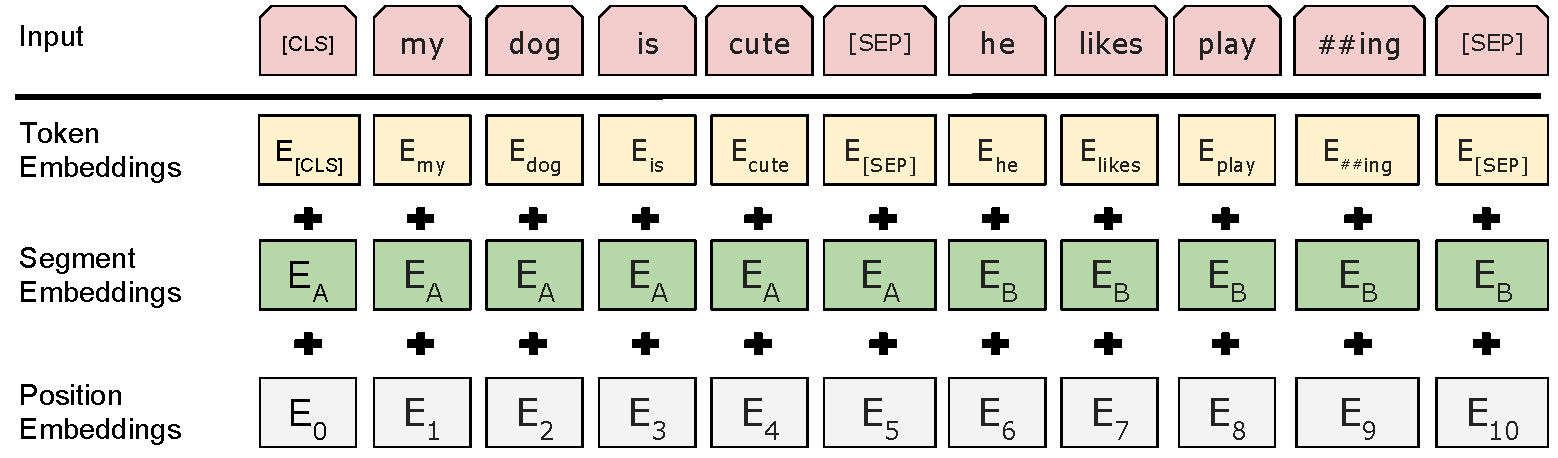
\includegraphics[width=.9\linewidth]{img/Input_Emebeddings.pdf}
\caption{\label{fig:inputemebeddings}Пример ввода текста в модель}
\end{figure}

При обучении модель выполняет на 2 задания:
\begin{enumerate}
\item Предсказание слова в предложении

Поскольку стандартные языковые модели либо смотрят текст слева направо или справа налево \ref{fig:BERT_comparisons}, как ELMo \autocite{elmo} и GPT \autocite{radford2019language}, они работают с контекстом хуже, чем данная модель. Так как BERT двунаправленный, у каждого слова можно посмотреть его контекст, что позволит предсказать замаскированное слово.

\begin{figure}[h]
\centering
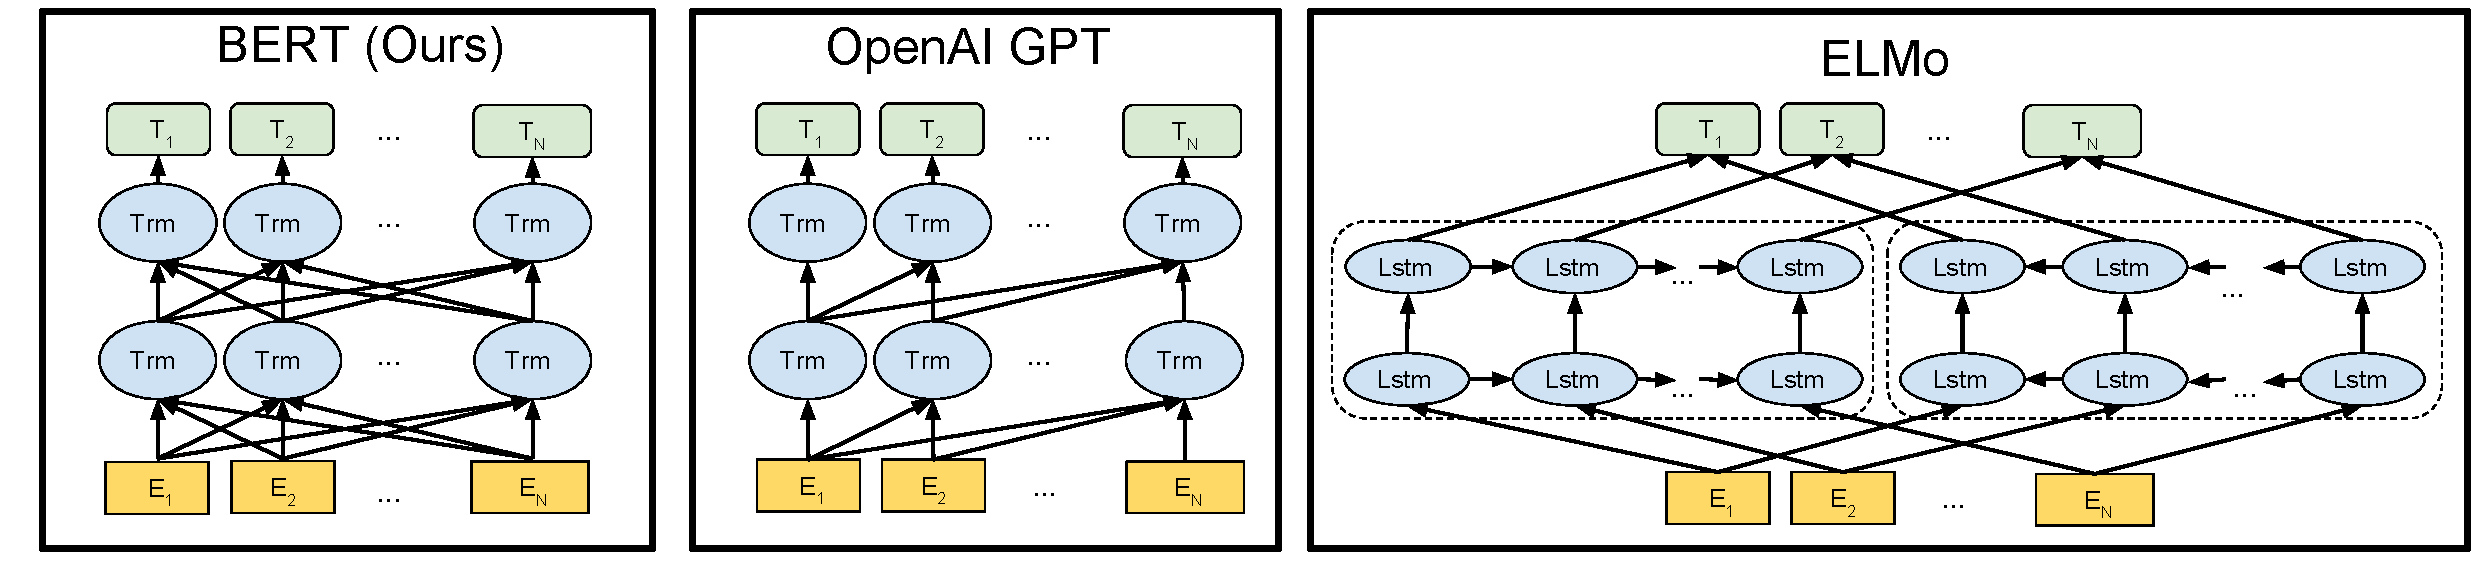
\includegraphics[width=.9\linewidth]{img/BERT_comparisons.pdf}
\caption{\label{fig:BERT_comparisons}Сравнение принципов работы BERT, ELMo, GPT}
\end{figure}

Это задание обучается следующим образом -- 15\% случайных слов заменяются в каждом предложении на специальный токен \texttt{[MASK]}, а затем предсказываются на основании контекста. Однако иногда слова заменяются не на специальны токена, в 10\% заменяются на случайный токен и еще в 10\% заменяются на случайное слово.

\item Предсказание следующего предложения

Для того чтобы обучить модель, которая понимает отношения предложений, она предсказывает, идут ли предложения друг за другом. Для этого с 50\% вероятностью выбирают предложения, которые находятся рядом и наоборот. Пример ввода пары предложений в модель \ref{fig:bert_pretrainin}.

\begin{figure}[!hbp]
\centering
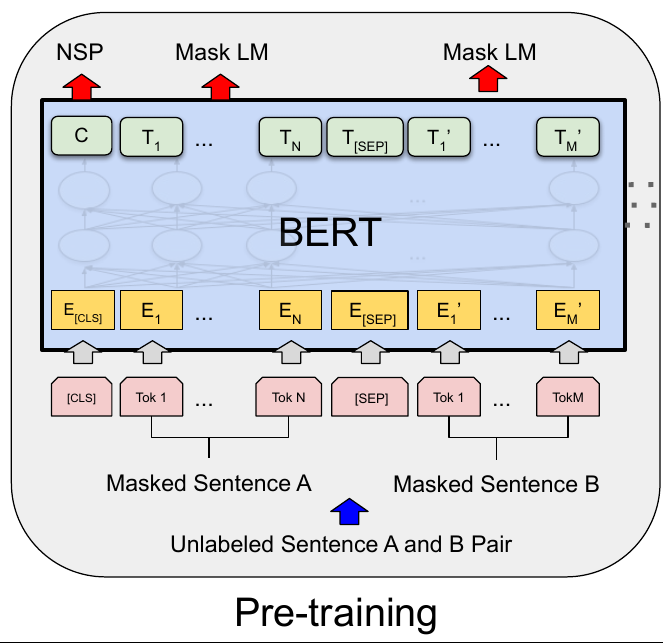
\includegraphics[width=0.6\textwidth]{img/bert_pretrainin.png}
\caption{\label{fig:bert_pretrainin}Схемам работы BERT}
\end{figure}
\end{enumerate}
\section{Sentense BERT}
\label{sec:orgbda5bd5}
Sentense BERT \autocite{reimers-2019-sentence-bert} -- это модификация предобученных моделей BERT, которая использует модель BERT и подает на вход 2 предложения, затем усреднят их выходы, а после с помощью функции ошибки выдаёт результат. Схема работы модели \ref{fig:sbert}.
\begin{figure}[hbp]
\centering
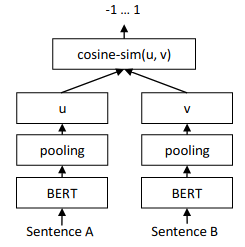
\includegraphics[width=0.4\textwidth]{img/sbert.png}
\caption{\label{fig:sbert}Схема работы SBERT}
\end{figure}
Основное преимущество данной модели над классическим BERT: эмбеддинги предложений можно сравнивать друг с другом независимо и не пересчитывать их пару каждый раз. Например, если для поиска похожих предложений из 10000 для обычного BERT потребуется 50 миллионов вычислений различных пар предложений, и это займёт 50 часов, то Sentense BERT рассчитает эмбеддинг каждого предложения отдельно и потом их сравнит, и это займёт примерно 5 секунд.
\section{CLIP}
\label{sec:org339bd3b}
CLIP (Contrastive Language–Image Pre-training)\autocite{radford2021learning} -- это нейронная сеть, обученная на множестве пар (изображение, текст). Его можно проинструктировать на естественном языке, чтобы он предсказал наиболее релевантный фрагмент текста, учитывая изображение, без прямой оптимизации для задачи. Эта модель состоит из двух разных моделей. Одна для кодирования текста в эмбеддинг -- трансформер \autocite{NIPS2017_3f5ee243}, а для кодирования изображения используется vision transformer \autocite{dosovitskiy2020image}. В данной работе будет использована модификация этого метода для сопоставления текстов из разных сфер между собой.

Метод обучения данной модели авторы отнесли к "natural language supervision" (обучение естественным языком). На каждой итерации обучения берется набор пар изображение-текст. Затем они трансформируются в эмбеддинги и к каждому тексту модель пытается подобрать текст, и наоборот. Данный способ позволяет соединить пространства двух различных источников информации.
\chapter{Проектирование системы}
\label{sec:orgf20e9f0}
\section{Проектирование базы данных}
\label{sec:org6e411fc}

\section{Проектирование архитектуры системы}
\label{sec:org4b21fc5}
\subsection{Проектирование серверной части}
\label{sec:orgfbf68c5}
\subsection{Проектирование клиентской части}
\label{sec:orgfd93481}

\chapter{Реализация системы}
\label{sec:org34a84ee}
\section{Реализация серверной части}
\label{sec:orgd5f43d7}
\subsection{Реализация API}
\label{sec:orgb704a29}
\subsection{Реализация парсера banki.ru}
\label{sec:org68a1c83}
\subsection{Реализация парсера sravni.ru}
\label{sec:orgbcd1bb6}
\subsection{Реализация модуля обработки текста}
\label{sec:org7bd4205}
\section{Реализация клиентской части}
\label{sec:orgbdf6fa6}
\chapter{Тестирование системы}
\label{sec:org3f42e0b}
\chapter*{Заключение}
\label{sec:org0833c48}
%\nocite{*}
\putbibliography
\appendix
\end{document}
